% 流域人水系统是典型的社会\textendash{}生态系统,系统演变机制是社会\textendash{}生态系统研究的核心内容。
% 根据侧重点的不同,武旭同将当前社会\textendash{}生态系统互馈的机制总结为“时”(系统弹性)、“空”(全程耦合)、“构”(结构匹配)、“阈”(地球界限)四个方面,其中“时”为包含弹性和稳态转换在内的一组概念,是研究社会\textendash{}生态系统动态演化的重要理论框架,对理解人水系统的演变机制至关重要\cite{WuXuTong2021}。
% 本节综述了与稳态转换密切相关的核心概念,并分别围绕“驱动因素、表现特征、级联效应”三个稳态转换的核心要素,总结了分析人水系统演变机制的主要路径。

\subsubsection{稳态转换与相关概念}

% 宋嘉熙 的 地理学报
弹性(Resilience)是指处于动态平稳的系统面对变化时通过缓冲、适应或转变等方式响应得以维持的能力\cite{folke2010}, 稳态转换(Regime shifts)指系统的结构和功能发生大规模重组并突破这种平稳状态的过程\cite{scheffer2001},在生态系统、气候系统、经济系统、及其它复杂系统中均可能发生,具有不易预测、难恢复的特点\cite{scheffer2003, biggs2009}。
通常使用“球-杯模型”或“折叠二分模型”来描述稳态转换。
以“球-杯模型”为例,不同稳态就像系统状态空间中凹陷的“杯子”,将系统实际状态则如同在不同凹陷间滚动的“小球”,状态空间的变化(参量驱动)或小球受到外力(变量驱动)时都可能推动系统状态在不同稳态间发生转换\cite{scheffer2009, folke2010}(图\ref{ch1:fig:regime_shift})。
稳态转换的诱发机制可以从参量驱动和变量驱动两个方面入手,前者是指外界条件(环境参数)发生变化时削弱系统弹性导致的稳态转换,后者是指系统内部或外部变量推动系统突破阈值从而触发的稳态转换\cite{scheffer2009, folke2010}(图\ref{ch1:fig:regime_shift})。
除了驱动因素外,系统稳态转换的发生可能致使系统功能与产出(Outcome)发生变化,或进一步触发其它的级联效应(Cascading Effect)\cite{rocha2018}。
因此,识别稳态转换应从“驱动力-现象-效应”这三个稳态转换的核心要素切入,从而厘清系统间反馈机理、分析关键要素间交互作用,揭示社会\textendash{}生态系统稳态转换的成因类型、现象特征与产出/外溢效应。

% Description of system regime shift by ball-cup model and fold bifurcation
\begin{figure}[!ht] % use float package if you want it here
    \centering
    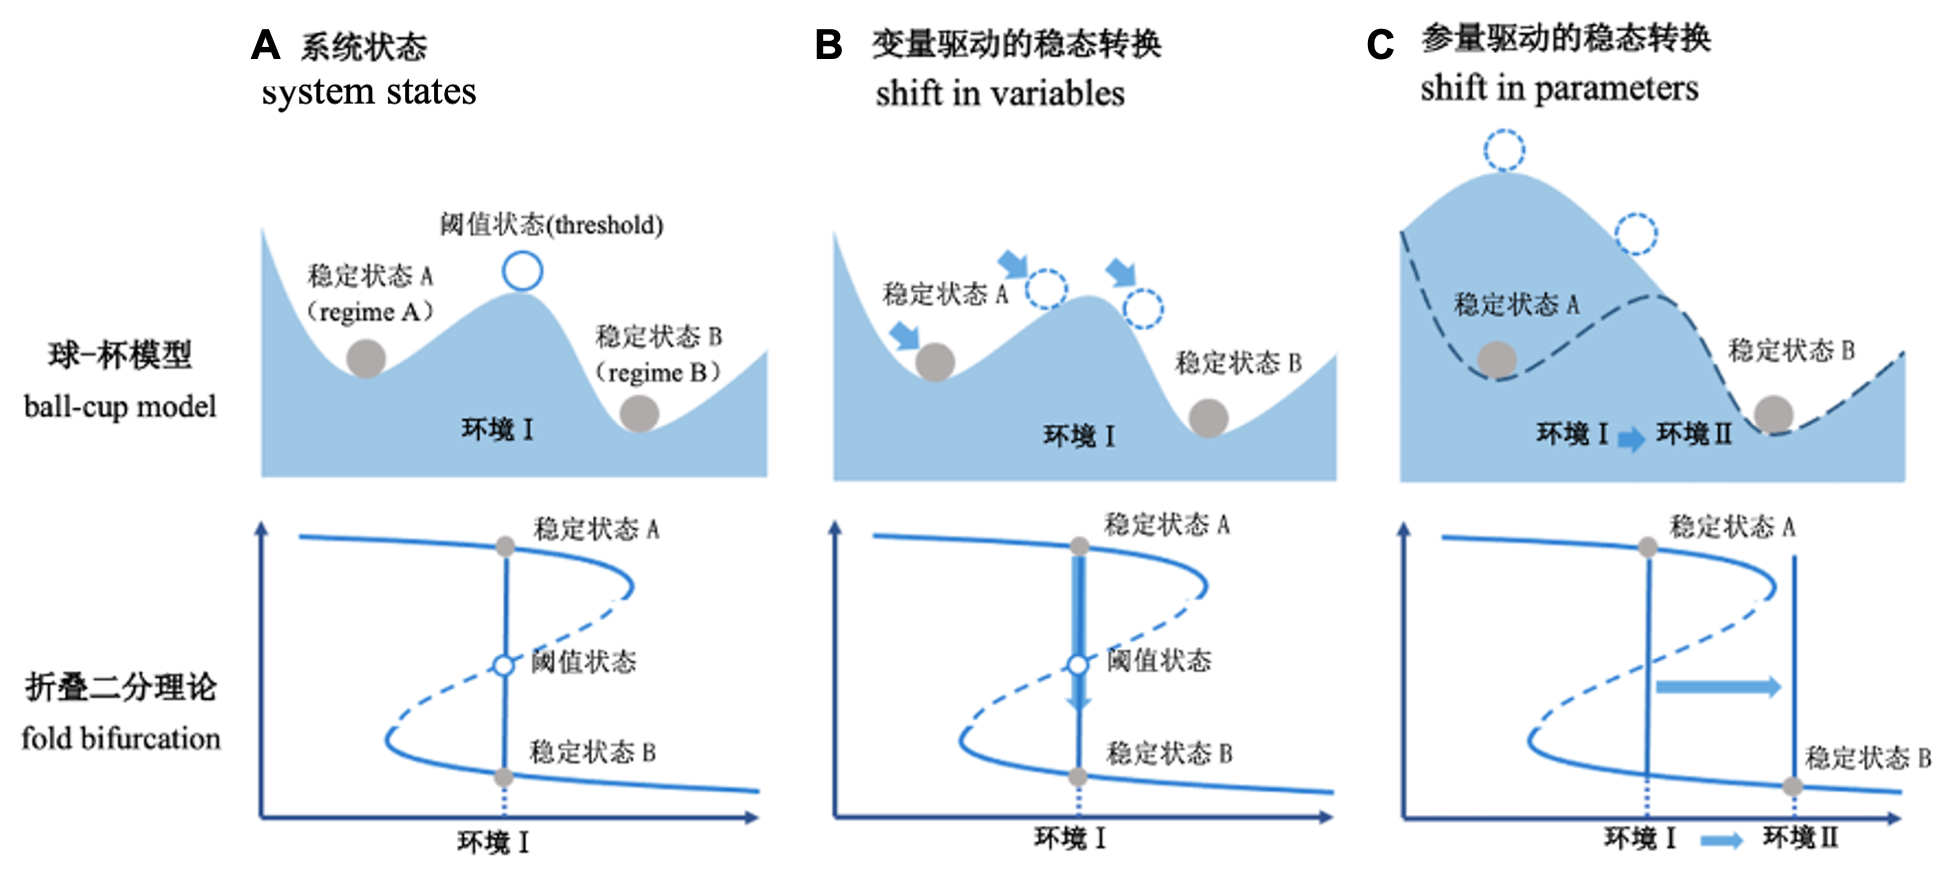
\includegraphics[width=\textwidth]{img/ch1/ch1_regime_shift.png}
    \caption[系统的稳态转换理论框架]{系统的稳态转换理论框架。
    \textbf{A}假设系统中存在稳定状态A和稳定状态B,球-杯模型(ball-cup model)和折叠二分理论(fold bifurcation)对系统各种状态的表征。
    \textbf{B}系统稳态转换过程。变量驱动的稳态转换(shift in variables):环境\romannumeral1不变时,处于稳定状态A的系统在干扰下自身突破阈值状态转换为稳定状态B。
    \textbf{C}参量驱动的稳态转换。环境\romannumeral1变为\romannumeral2,迫使处于稳定平衡状态A的系统向新环境下仅存的稳定平衡状态B转换。}\label{ch1:fig:regime_shift}
\end{figure}

\subsubsection{稳态转换的驱动因素}

Rocha等人发现,不断累积的人为干扰压力和气候变化是最常见的两类稳态转换驱动因素,无论以变量还是参量的形式出现\cite{rocha2018}。
Ji等根据水-沙调节方案和河口河道迁移这两个主要驱动因素变化的时间节点,结合不同阶段河口侵蚀-沉积量与河口排沙量,确定了河口侵蚀-积聚模式的稳态转换过程\cite{ji2018}。
Bao等在分析黄河中游水平衡系统稳态转换时,识别出气候驱动因素和土地利用/覆盖显著变化的阶段。通过验证不同阶段水平衡状态的差异确定了不同稳态阶段,并进一步定量解析了驱动水平衡状态转换的具体机制\cite{bao2019}。
此类分析路径的关键在于准确选择系统驱动力的定量表征,因此需要预设系统稳定状态和驱动力之间的关系。
这种方法多用于驱动力易于识别的干扰因素,如持续减少的林地、持续周期性变化的气候等。

“稳态循环”理论有助于理解另一类常见的人为干扰——流域治理措施——驱动的稳态转换。
该理论认为系统在不同尺度下都可以自组织历经适应性循环的“开发”、“保护”、“释放”、“更新”四个阶段\cite{gunderson2001},之后又进一步总结为“涌现”、“制度化”、“更新”三个阶段。
基于“主动改变不良的社会\textendash{}生态系统状态”与“调节并维持良好的社会\textendash{}生态系统状态”两种不同的目的,治理措施可分为自上而下的“转型治理”和自下而上的“协作治理”两类\cite{song2019}。
转型治理关注社会\textendash{}生态系统的释放和更新阶段,强调适应性治理的实现和主动促使社会\textendash{}生态系统完成状态的更新;协作治理则强调适应性治理制度化过程,旨在通过利益相关者间自组织的协作模式来实现社会\textendash{}生态系统的开发与保护\cite{song2019}。
因为无论自上而下或自下而上,流域治理既可能维持稳态,也可能触发稳态转换,需要在分析流域治理措施的作用机制时加以甄别。

\begin{figure}[!ht] % use float package if you want it here
    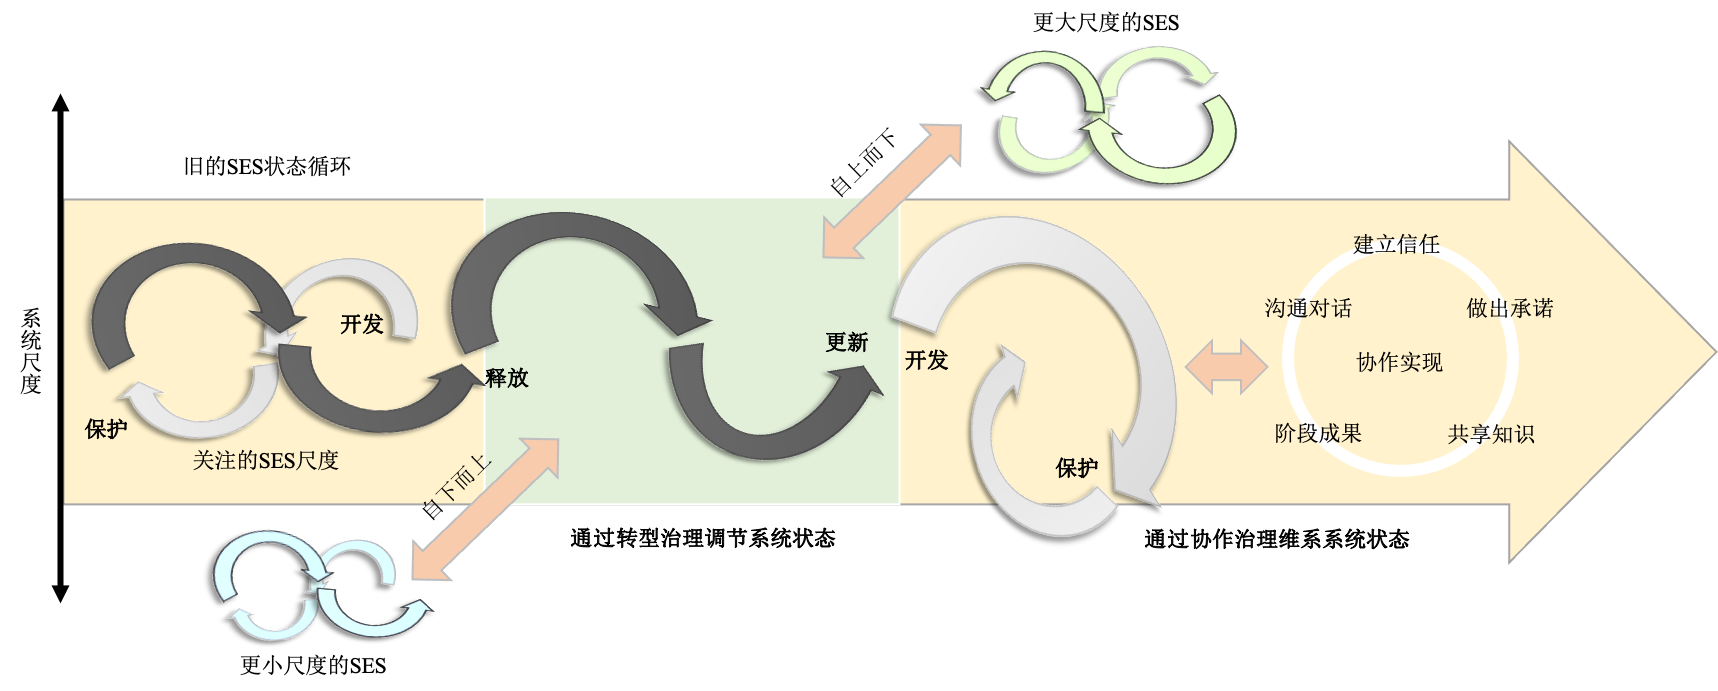
\includegraphics[width=\textwidth]{img/ch1/ch1_governance_driver.png}
    \caption[社会\textendash{}生态系统状态循环]{社会\textendash{}生态系统状态循环与转型治理、协作治理的关系。
    % Fig.4  The relationship between social-ecological system adaptive cycle and transition / collaborative governance
    图中展示旧的社会\textendash{}生态系统(SES)因转型治理而进入新的状态循环,并因协作治理的实现而延长开发保护阶段的过程}\label{ch1:fig:governance_driver}
\end{figure}

\subsubsection{稳态转换的表现特征}

聚焦于稳态转换过程中所表征出的现象是分析稳态转换最常见的路径,通过寻找合适的指标识别系统互馈变量或相关解释变量的趋势突变,检测稳态转换现象。
相关的检测方法非常丰富,常见的包括趋势分析、突变点检测或断点回归等。
Wang等利用t检验的循序算法和加性季节和趋势断点模型两种方法检测$1950 \textendash{} 2011$年黄河流域上中下游径流和输沙量的突变时间点以确定稳态转换时期\cite{wang2014};
Zhao等利用曼-肯德尔(Mann-Kenall)趋势分析法和加性季节和突变点检测模型识别出1921—2011年期间黄河月径流量趋势突变,重建天然径流量,量化人类活动对流量稳态转换的影响程度\cite{zhao2015}。

在识别稳态转换现象的基础上,还可以进一步将其与稳态转换驱动力相关联。
Yang等利用 Pettitt 检验计算稳态转换指数,探测流域径流的稳态转换,并与气候和土地利用变量的突变点对比分析,证实土地利用政策驱动了径流的稳态转换\cite{yang2012a}。
Niu等检测了黄河三角洲系统降水量,温度,月径流量和归一化植被指数(Normalized Difference Vegetation Index,NDVI)等多个现象相关变量共同的分解趋势断点,识别水文\textendash{}气候\textendash{}植被系统的稳态转换时期,分析各阶段内气候水文变量与NDVI间产出效应\cite{niu2020}。
虽然聚焦于稳态转换现象表征易于直观划分稳态转换的时期,且有着成熟的数据检测技术,但如果忽略对驱动和效应的结合分析,容易对稳态转换的驱动-响应机制表达不够全面。

\subsubsection{稳态转换的级联效应}

级联效应是指系统稳态转换后所产生的一系列后续影响,通过分析级联效应,可以更好地理解系统内部互馈关系的复杂性\cite{rocha2018}。
根据受到影响的要素在系统内或系统外,级联效应可分为内联效应和外溢效应\cite{rocha2018}。
在研究稳态转换时,Sun等利用沉积率曲线参数变化来刻画泥沙运输稳态转换的产出效应变化特征,同时解释了生态恢复对泥沙运输稳态的调节作用\cite{sun2020};
Wu等在研究黄土高原社会\textendash{}生态系统稳态转换时,通过量化社会\textendash{}生态系统内部要素交互作用的稳定状态,揭示了稳态转换不同阶段内系统关系变化和外溢效应\cite{wu2020a}。
Kidder等在研究黄河河道泥沙淤积系统稳态转换时,利用外溢系统中黄河下游洪水的频率和规模变化确定稳态转换发生时期,指出堤坝作为驱动因素对泥沙淤积存在着强烈正反馈\cite{kidder2015}。
此类分析路径有助于识别复杂的社会\textendash{}生态系统稳态转换的发生机制,正成为稳态转换实证研究的热点,但需要准确选择与系统反馈过程联系紧密的级联现象,因此也需要关于系统稳态的先验知识。

总的来说,虽然已有很多研究从驱动因素、表现特征和级联效应等不同方面探究人水系统的稳态转换机制,并提出了相应的量化方法,但稳态转换是大规模的系统重组,需要考虑多个要素的同步变化。
仅从单一要素出发的研究容易导致对其机制认识不全面,因此需要进行系统整合,探讨“驱动-现象-效应”的多要素联合变化。
